% \documentclass[12pt]{article} % increase font size
\documentclass[a4paper,12pt]{book}

\usepackage{hyperref}
\usepackage{listings}
\usepackage{graphicx}
\usepackage{xcolor}
\usepackage{amsmath}
\usepackage{amssymb}
\usepackage{amsthm}
\usepackage{enumitem}
\usepackage{tikz}
\usepackage{circuitikz}
\usepackage{pgfplots}
\usepackage{float}
\usepackage{subcaption}
\usepackage{geometry}
\usepackage{fancyhdr}
\usepackage{lastpage}
\usepackage{multicol}
\usepackage{multirow}
\usepackage{tabularx}
\usepackage{booktabs}
\usepackage{longtable}
\usepackage{array}
\usepackage{makecell}
\usepackage{siunitx}
\usepackage{url}
\usepackage{pdfpages}
\usepackage{verbatim}
\usepackage{wrapfig}
\usepackage{tcolorbox}
\usepackage{csquotes}
\usepackage{calc}
% transparent colors for tikz
\usepackage{transparent}
\input{arduinoLanguage.tex}    % adds the arduino language listing

\geometry{a4paper, top=25mm, left=20mm, right=20mm, bottom=25mm}

% Warning box
\newtcolorbox{warning}[1][]
{
  colframe=yellow!50!red,
  colback=yellow!30,
  coltitle=red!20!black,
  title={Achtung!},
  #1
}

\newtcolorbox{instruction}[1][]
{
  colframe=cyan!50!blue,
  colback=cyan!40,
  coltitle=blue!20!black,
  title={Jetzt Du!},
  #1
}

\newcommand{\hrefnote}[2]{\href{#1}{#2}\footnote{\url{#1}}}
\newcommand{\hrefnoteinline}[2]{\href{#1}{#2} (\url{#1})}

%% Define an Arduino style fore use later %%
\lstdefinestyle{myArduino}{
  language=Arduino,
  %% Add other words needing highlighting below %%
  morekeywords=[1]{},                  % [1] -> dark green
  morekeywords=[2]{FILE_WRITE},        % [2] -> light blue
  morekeywords=[3]{SD, File},          % [3] -> bold orange
  morekeywords=[4]{open, exists},      % [4] -> orange
  %% The lines below add a nifty box around the code %%
  frame=shadowbox,
  rulesepcolor=\color{arduinoBlue},
}

\lstMakeShortInline[style=myArduino]|
\lstset{style=myArduino}

% Patch from https://tex.stackexchange.com/questions/451532/recent-issues-with-lstlinebgrd-package-with-listings-after-the-latters-updates
\makeatletter
\let\old@lstKV@SwitchCases\lstKV@SwitchCases
\def\lstKV@SwitchCases#1#2#3{}
\makeatother
\usepackage{lstlinebgrd}
\makeatletter
\let\lstKV@SwitchCases\old@lstKV@SwitchCases

\lst@Key{numbers}{none}{%
    \def\lst@PlaceNumber{\lst@linebgrd}%
    \lstKV@SwitchCases{#1}%
    {none:\\%
     left:\def\lst@PlaceNumber{\llap{\normalfont
                \lst@numberstyle{\thelstnumber}\kern\lst@numbersep}\lst@linebgrd}\\%
     right:\def\lst@PlaceNumber{\rlap{\normalfont
                \kern\linewidth \kern\lst@numbersep
                \lst@numberstyle{\thelstnumber}}\lst@linebgrd}%
    }{\PackageError{Listings}{Numbers #1 unknown}\@ehc}}
\makeatother

% https://tex.stackexchange.com/questions/8851/how-can-i-highlight-some-lines-from-source-code


\newcommand{\sidebyside}[1]{
\begin{minipage}{.5\textwidth}
  \begin{center}
    \includegraphics[width=.8\textwidth,
        % cut 1 cm from the bottom
        trim=0 .5cm 0 0, clip
    ]{schaltung/#1/#1_schem.png}
  \end{center}
\end{minipage}%
\begin{minipage}{.5\textwidth}
  \begin{center}
    \includegraphics[width=.8\textwidth,
        % cut 1 cm from the bottom
        trim=0 0.5cm 0 0, clip
    ]{schaltung/#1/#1_bb.png}
  \end{center}
\end{minipage}
}

\begin{document}


\title{Arduino Projekt}
\author{Marcel}
\date{}

% \maketitle


\section*{Einführung}

\begin{center}
\includegraphics[width=.8\textwidth]{images/material2.png}
\end{center}

\section*{Materialien}
\begin{multicols}{2}
\begin{enumerate}[label=\arabic*)]
  \item Arduino Nano (Prozessor: ATMega328P (Old Bootloader), Programmierschnittstelle: AVRISP mkII)
  \item Breadboard (Steckbrett)
  \item Kabel
  \item Potentiometer
  \begin{enumerate}
    \item Gehäuse 
    \item Drehknauf
    \item Druckstecker
  \end{enumerate}
  \item Zusammengebauter Potentiometer
  \item LED Band
  \item Kommerzielles Potentiometer
  \item Widerstände
  \begin{enumerate}
    \item $\SI{470}{\ohm}$ Widerstand
    \item $\SI{1}{\kohm}$ Widerstand
    \item $\SI{10}{\kohm}$ Widerstand
  \end{enumerate}
  \item Kondenstor
  \item Druck-Schalter
  \item $\SI{20}{\kohm}$ Widerstand
  \item LED
\end{enumerate}
\end{multicols}

Weiterhin benötigt:
\begin{itemize}
  \item Computer zum Programmieren
  \item Bleistift (idealerweise 2B)
  \item Doppelseitiges Klebeband
\end{itemize}

\section*{Breadboard}

\begin{center}
\includegraphics[width=.8\textwidth]{images/breadboard.jpg}
\end{center}

Ein Breadboard ist ein nützliches Werkzeug, um Schaltungen zu testen, ohne sie löten zu müssen.  
Es besteht aus einer Matrix von Löchern, die in Reihen und Spalten angeordnet sind.  
Die Reihen sind vertikal und die Spalten sind horizontal verbunden.

Am oberen und unteren Rand des Brettes befinden sich zwei Reihen.
Diese Reihen sind für die Stromversorgung vorgesehen.
Rot steht normalerweise für $V_{cc}$ und schwarz für GND.
Hierbei ist $V_{cc}$ die Spannungsversorgung (üblicherweise $5V$) und GND die Masse.

Der Vorteil der Reihen ist, dass man einfach Verbindungen in der Mitte des Breadboards mit Strom versorgen kann.

Die einzelnen Spalten sind alle getrennt.
Dies erlaubt es Verbindungen zwischen Komponenten herzustellen.
Innerhalb einer Spalte sind alle Löcher miteinander verbunden.
Über die Mitte besteht keine Verbindung.
Die meisten Bauteile sind so konzipiert, dass ihre Anschlüsse genau dem Abstand im Breadboard entsprechen.

Knöpfe passen in die Mitte des Breadboards zwischen zwei Spalten.

\section*{Arduino Nano Hardware Grundlagen}

Der GND Pin ist dauerhaft und permanent mit der Masse verbunden.
Der +5V Pin ist dauerhaft und permanent mit der Spannungsversorgung verbunden.
Wir benötigen keine zustätzliche Software oder Firmware.

Es gibt noch einen Haufen anderer Pins wie 3V3 für eine 3V Spannungsversorgung, A0 bis A7 für analoge Eingänge, und D0 bis D13 für digitale Ein- und Ausgänge.
Zustäzlich gibt es einen zweiten GND Pin, der ebenfalls mit der Masse verbunden ist.
Die anderen Pins sind für spezielle Funktionen reserviert.

\section*{Probiere es aus! LED}
% Arduino in Breadboard, LED drin

\begin{wrapfigure}{r}{5cm}
  \begin{minipage}{.3\linewidth}
    \begin{circuitikz}
      \draw (0,0) node[ground]{} to[short] (0,0) to[leD] (0,1) to[short] (0,1) node[vcc]{};
    \end{circuitikz}
  \end{minipage}%
  \begin{minipage}{.69\linewidth}
  \includegraphics[width=3cm]{images/led.png}
  \end{minipage}
\end{wrapfigure}

% \begin{wrapfigure}{r}{3cm}
%   \centering
%   \includegraphics[width=3cm]{images/led.png}
% \end{wrapfigure}

Jetzt wollen wir einfache Anschlüsse ausprobieren.
Dazu wollen wir eine LED mit Hilfe des Stromes vom Arduino Nano zum Leuchten bringen.

Eine LED (Light Emitting Diode) ist ein Halbleiterbauelement, das Licht emittiert, wenn ein elektrischer Strom durch sie hindurch fließt.

Die LED hat ein kurzes und ein langes Bein.
Das kurze ist die Kathode (Minuspol) und das lange die Anode (Pluspol).

Als ersten Schaltkreis zum Kennenlernen, wollen wir die LED mit der Stromversorgung des Arduino Nano verbinden.
Dazu verbinden wir 5V zur Anode der LED und die Kathode über einen Widerstand mit GND.
Hierbei ist es prinzipiell egal, ob der Widerstand vor oder nach der LED geschaltet wird.

Dies sind drei Schaltpläne für diese Schaltung auf unterschiedlichen Beschreibungsebenen:

% \begin{figure}[!ht]
\begin{center}
  \includegraphics[width=.49\textwidth]{schaltung/led/circuit.png}

  \includegraphics[width=.49\textwidth]{schaltung/led/scheme.png}
  \includegraphics[width=.49\textwidth]{schaltung/led/scheme2.png}

  \includegraphics[width=.70\textwidth]{schaltung/led/foto.jpg}%
\end{center}
% \end{figure}
Die erste Schaltung stellt ein Schaltbild, wie du es aus Physik kennst, dar.
Hierbei sind die Verbindungen abstrakt als Linien gekennzeichnet und die Bauteile als 
\hrefnote{https://de.wikipedia.org/wiki/Schaltzeichen}{Schaltzeichen}.
Diese Variante ist die universelle Variante zum Austausch über Schaltungen und wird generell verstanden.
Zudem kann man diese Variante auch einfach per Hand zeichnen.

Die zweite Version ist eine abstrahierte Repräsentation der Schaltung.
Hierbei sind Kabel wie physisch vorhanden dargestellt und die Bauteile als einfache Formen.
Es ist klarer verständlich als das Schaltbild, aber weniger universell (wie dargestellt durch zwei Varianten).
Diese Variante eignet sich gut zur konkreten Kommunikation insbesondere am Anfang.
Sie wird meist in Simulatoren verwendet, um Schaltungen durchzuspielen.

Die letzte Variante ist ein Foto der physischen Schaltung.
Durch Perspektive, Lichtverhältnisse, Farben und Kabellängen sind Details
hier meist schwer zu erkennen.

Siehe die Referenzen für Programme und Webseiten, um Schaltpläne zu erstellen
und digital mit Schaltungen zu arbeiten.

Eine weitere Möglichkeit ist, die Schaltung auf einer Platine zu bauen.
Dafür erstellt man ein PCB (Printed Circuit Board).
In eine Kupferplatte werden die Leiterbahnen geätzt und die Bauteile darauf gelötet.
Die Schaltung gibt an, wo Löcher im PCB gebohrt werden müssen, um die Bauteile zu befestigen,
und wo die Leiterbahnen verlaufen.
Ähnlich zu Steckbrettern gibt es auch Steckplatinen, auf denen die Bauteile eingesteckt werden können.
Im Folgenden Bild ist der rechte PCB nur ein Beispiel für eine fertige Platine.
\begin{center}
  \includegraphics[width=.49\textwidth]{schaltung/led/pcb.png}%
  \includegraphics[width=.49\textwidth]{images/pcb.jpg}%
\end{center}


\begin{warning}
  Achte darauf, dass ein Widerstand in Reihe mit der LED geschaltet ist.
  Andernfalls kann die LED durchbrennen und der Arduino Nano beschädigt werden.

  Zwischen VCC und GND sollte niemals eine direkte Verbindung bestehen, da dies einen Kurzschluss verursachen würde.
  Sorge immer dafür, dass ein Widerstand zwischen möglichen Verbindungen von VCC und GND besteht.

  Bei anderen Pins wie den analogen Pins ist eine Verbindung zu VCC kein Problem, da diese über einen internen Widerstand verfügen.
\end{warning}

\begin{instruction}
  Probiere es selbst aus:
  \begin{enumerate}
    \item Platziere den Arduino Nano im Breadboard.
    \item Verbinde den Arduino Nano schonmal mit dem Computer.
    \item Verbinde die Anode der LED mit dem 5V Pin des Arduino Nano.
    \item Verbinde die Kathode der LED mit einem Widerstand.
    \item Verbinde den anderen Anschluss des Widerstands mit dem GND Pin des Arduino Nano.
  \end{enumerate}

  Was passiert wenn wir die LED umdrehen?
\end{instruction}




\section*{Arduino Nano Software Grundlagen}

Jetzt, da wir Strom haben und unsere erste Schaltung auf dem Schaltbrett aufgebaut haben, wollen wir den Arduino Nano programmieren.
Dazu müssen wir ihn erst einmal einrichten.

Lade die Arduino IDE von \url{https://www.arduino.cc/en/software} herunter.
Wähle dazu \enquote{Win 10 and newer, 64bit} aus, dann \enquote{Just download}.
Nach der Installationen beziehungsweise beim ersten Öffnen, musst du die Dienste
zulassen und gegebenenfalls Treiber installieren.

\begin{minipage}{.5\textwidth}
\begin{center}
\includegraphics[height=7cm]{images/ide.png}%
\end{center}
\end{minipage}
\begin{minipage}{.5\textwidth}
\begin{center}
\includegraphics[height=7cm]{images/ide_port.png}
\end{center}
\end{minipage}

Verbinde den Arduino Nano mit dem Computer falls noch nicht geschehen.
Wähle als Barod \enquote{Arduino Nano} aus, wähle den Bootloader \enquote{ATmega328P (Old Bootloader)} und wähle den Port aus.
Falls mehrere Ports (COM Ports unter Windows) angezeigt werden, probiere einfach aus, welcher der richtige ist.
Sollte eine \enquote{Zugriff verweigert} Meldung kommen, versuche die IDE als Administrator zu starten.

Danach solltest du über den Upload Button (Pfeil nach rechts) den Code auf den Arduino Nano übertragen können.

Auf dem Arduino Nano sind vier LEDs verbaut:
\begin{itemize}
  \item RX (Receive) --- blinkt beim Hochladen von Code (verbunden mit dem RX0 Pin)
  \item TX (Transmit) --- blinkt bei serieller Kommunikation (verbunden mit dem TX0 Pin)
  \item PWR (Power) --- leuchtet wenn der Arduino Nano mit Strom versorgt wird
  \item L (Load) --- blinkt beim Starten des Programms (verbunden mit dem D13 Pin)
\end{itemize}

Jetzt können wir uns den Code anschauen.

\begin{lstlisting}
void setup() {
  // put your setup code here, to run once:
}

void loop() {
  // put your main code here, to run repeatedly:
}
\end{lstlisting}

Dieser Code ist der leere Standard Code, der beim Öffnen der Arduino IDE angezeigt wird.
Üblicherweise nutzt man C++ als Programmiersprache für den Arduino Nano.
Wir nutzen C++ in der Arduino Nano IDE, die das Kompilieren (Übersetzen) und Hochladen des Codes auf den Arduino Nano übernimmt
und Teile des C++ Codes für uns schreibt.

Im leeren Programm sind bereits zwei Funktionen vorhanden: |setup| und |loop|.
Die |setup| Funktion wird einmalig beim Start des Programms ausgeführt.
Hier initialisieren wir Variablen und setzen Pins auf Ein- oder Ausgänge.
Die |loop| Funktion wird immer wieder ausgeführt.
Hier schreiben wir den Hauptteil unseres Programms.

Die IDE dürfte dir vielleicht bekannt vorkommen.
Sie ist ähnlich zu Processing, einer Programmiersprache für Zeichnen, Animation und Interaktion, 
die auf Java basiert.

Die Details wie serielle Kommunikation, Bibliotheken und Beispiele werden wir uns später anschauen.

\section*{Serielle Kommunikation}
Prinzpiell steht der Arduino allein da.
Man kann ihn mit einer Batterie, Akku, Powerbank, Ladekabel, \ldots betreiben
und er kann selbstständig Aufgaben ausführen.
Der Mikrocontroller ist in sich abgeschlossen.

Die Verbindung zum Computer wird lediglich zum Programmieren und Debuggen benötigt.
Zum Debuggen ist es nützlich, wenn der Arduino mit uns kommunizieren kann.
Das geht über die serielle Kommunikationsschnittstelle.

\lstinputlisting{programs/communication/communication.ino}

Zuerst müssen wir dem Arduino Nano sagen, dass wir die serielle Kommunikationsschnittstelle nutzen wollen.
Das machen wir in der |setup| Funktion mit |Serial.begin(9600)|.
Die Zahl gibt die Baudrate an, also die Geschwindigkeit der Kommunikation.
Danach können wir mit |Serial.println("Hello World")| eine Nachricht an den Computer senden.
Diese wird im Seriellen Monitor der Arduino IDE angezeigt.

In der Schleife |loop| wird eine Nachricht immer wieder gesendet.
Wir warten zwischen jeder Nachricht $\SI{2000}{\milli\second}$, also zwei Sekunden.

Du siehst, dass jede Zeile wie in C\# mit einem Semikolon endet.

\begin{instruction}
  Probiere es selbst aus:
  \begin{enumerate}
    \item Lade den Code auf den Arduino Nano.
    \item Öffne das Serielle Monitor (rechts oben auf das Lupe Symbol klicken).
    \item Was passiert, wenn du den Reset Knopf drückst?
  \end{enumerate}
\end{instruction}

Wir können auch Variablen erstellen.
Lassen wir den Arduino mal Schafe zählen.
Da wir über die Schleifen hinweg zählen wollen, müssen wir die Variable außerhalb der |loop| Funktion deklarieren.
Schreiben wir also ganz oben |int count = 0;|, um eine Variable |count| zu erstellen und auf $0$ zu setzen.

In der |loop| Funktion können wir dann |count| erhöhen und ausgeben.
Wenn über |Serial.print| können wir entweder einen festen Text oder eine Variable ausgeben.
Mit |Serial.println| wird automatisch ein Zeilenumbruch am Ende hinzugefügt (bei |print| nicht).

% hightlight line 1, 9, 10
\lstinputlisting[
  linebackgroundcolor={
    \ifnum\value{lstnumber}=1\color{green!20}%
    \else\ifnum\value{lstnumber}=9\color{green!20}%
    \else\ifnum\value{lstnumber}=10\color{green!20}%
    \fi\fi\fi
  }
]{programs/count/count.ino}

\begin{instruction}
  \enquote{1 Schafe} ist kein richtiges Deutsch.
  Wie kann man das beheben?
\end{instruction}


\section*{(Analog) Lesen}
Wir wollen uns zuerst mit Lesen von auf Pins beschäftigen.
Dafür bauen wir eine Potential Schaltung.

\sidebyside{resistors}

Unsere Schaltung hat zwei Widerstände zwischen $V_{cc}$ und GND.
Wir wollen die Spannung an verschiedenen Punkten messen.
Für eine Messung verbinden wir unseren Pin, hier der analoge Pin A0, mit dem Punkt, an dem wir messen wollen.
Wir schauen uns dann an, was für Strom, genauer gesagt, wie viel Spannung, über unseren Pin abgegriffen wird.

Zuerst schreiben wir den Code, der die Spannung misst und uns mittels der seriellen Kommunikationsschnittstelle ausgibt.
\lstinputlisting{programs/read_a0/read_a0.ino}
Den Wert des Pins bekommen wir über |analogRead(A0)|.
|A0| ist eine vordefinierte Konstante für den analogen Pin 0.
Der Wert liegt zwischen $0$ und $1023$.

\begin{instruction}
  Probiere es selbst aus:
  \begin{enumerate}
    \item Baue die Schaltung auf.
    \item Lade den Code auf den Arduino Nano.
    \item Öffne das Serielle Monitor.
    \item Was passiert, 
    \begin{enumerate}
      \item wenn du zwischen den Widerständen misst?
      \item wenn du vor dem ersten Widerstand misst?
      \item wenn du nach dem zweiten Widerstand misst?
      \item einen der Widerstände austauschst?
      \item in der Luft/an deinem Finger misst?
    \end{enumerate}
  \end{enumerate}
\end{instruction}

Führe erst die Experimente oben durch sonst wird dir die Lösung vorgesagt.
Wenn kein Pfad zwischen dem Pin und Vcc oder GND besteht, wird der Pin schwanken.
Man bezeichnet diesen Zustand als floating.
Dies kann zu ungenauen Messungen führen. Insbesondere mit Schaltern und bei langen Kabeln 
muss man daher auf eine klare Verbindung achten.
Hier nutzt man sogenannte \hrefnote{https://en.wikipedia.org/wiki/Pull-up_resistor}{Pullup/Down Widerstände}\footnote{Siehe auch das Konzept einer \hrefnoteinline{https://de.wikipedia.org/wiki/Open_circuit}{offenen Schaltung}.}

Im Folgenden (und allgemein) benutzen wir gedankliche Modelle, die nicht der Realität entsprechen, 
aber nützlich zum Verständnis sind.

Vor dem ersten Widerstand kann der ganze Strom direkt von VCC zu A0 fließen.
Daher sehen wir den maximalen Wert von $1023$.
Nach dem zweiten Widerstand kann der ganze Strom direkt von A0 zu GND abfließen.
A0 ist geerdet beziehungsweise auf GND gezogen und wir sehen den minimalen Wert von $0$.
Zwischen den Widerständen teilt sich der Strom auf gleichmäßig auf.
Wir sehen einen Wert in der Mitte von circa $510$.

\section*{Schreiben auf (Digital) Pins}
% LED per Pin anschalten, D4
% pinMode
Wir können jetzt Werte lesen. Aber wir wollen auch Dinge ausgeben.

Dazu schauen wir uns die digitalen Pins an.
Bisher haben wir nur analoge Pins genutzt. Diese Pins sind A0 bis A7
und befinden sich auf der Seite mit +5V.

Die digitalen Pins sind D2 bis D13 und befinden sich meist (bis auf D13) auf der anderen Seite.
D13 hat spezielle Funktionen und ist mit der LED L verbunden.

Der Unterschied zwischen digitalen und analogen Pins ist, dass analoge Pins einen speziellen A/D Wandler (analogue-to-digital) haben.
Sie haben damit alle Funktionalität von digitalen Pins und können zusätzlich analoge Werte lesen.

Digitale Pins haben zwei Zustände: HIGH (3.3 oder 5V je nach Arduino) und LOW (0V).
Ähnlich zu der |analogRead| Funktion gibt es die |digitalRead| und |digitalWrite| Funktionen.

\lstinputlisting{programs/write/write.ino}

Wenn wir einen Pin als Ausgang nutzen wollen, müssen wir ihn zuerst als Ausgang definieren.
Das geschieht über die |pinMode| Funktion.
Mit |pinMode(2, OUTPUT)| definieren wir den Pin D2 als Ausgang.
Bemerke, dass die analogen Pins A0 bis A7 als Bezeichner nutzen und die digitalen Pins nur Zahlen von 2 bis 13.
Standardmäßig sind die Pins als Eingang definiert.

Wenn wir den Pin D2 als Ausgang definiert haben, können wir ihn über |digitalWrite(2, HIGH)| auf HIGH setzen
und damit Strom fließen lassen.

\sidebyside{write}

Zum Testen, verbinden wir den Pin D2 mit einer LED und einem Widerstand.
Allgemein empfiehlt es sich hinter Ausgabe Pins einen $\SI{470}{\ohm}$ oder $\SI{1}{\kohm}$ Widerstand zu schalten.
Ohne kann es gut gehen, aber man kann auch den Pin oder die LED beschädigen.

\begin{instruction}
  Probiere es selbst aus:
  \begin{enumerate}
    \item Baue die Schaltung auf.
    \item Lade den Code auf den Arduino Nano.
  \end{enumerate}
  Die LED ist sehr hell.
  \begin{itemize}
    \item Was passiert, wenn du den Widerstand durch einen größeren austauschst?
          Warum passiert das?
  \end{itemize}
\end{instruction}

Du hast bemerkt, dass größere Widerstände die LED dunkler machen.
Das liegt daran, dass weniger Strom fließt.
Die Erklärung liegt in $R = \frac{U}{I}$ oder genauer $I = \frac{U}{R}$.
Ein größerer Widerstand bedeutet weniger Strom bei gleicher Spannung.
Erinnere dich, dass in Reihe geschaltete Widerstände sich addieren.

Mit dem Potentiometer werden wir später einen bequemen Weg sehen den Widerstand zu steuern
und somit einen Dimmer zu bauen.

Ein anderer Weg, die Helligkeit zu steuern, ist die Pulsweitenmodulation (PWM).
Dabei wird der Pin schnell an und ausgeschaltet.

\begin{instruction}
  Probiere es selbst aus:
  \begin{enumerate}
    \item Ändere den Code so, dass der Pin D2 per PWM angesteuert wird.
    Statt für $\SI{1000}{\milli\second}$ HIGH wollen wir die LED 100mal für $\SI{1}{\milli\second}$ an und für $\SI{9}{\milli\second}$ aus schalten.
    Das entspricht circa $\SI{10}{\percent}$ Helligkeit.
    \item Per Auge nimmst du keine Unterschiede wahr. Was erkennst du auf deiner Handy-Kamera?
    \item Lade nochmal den alten Code hoch und vergleiche das Handy-Bild. Nun betrachte andere Lichtquellen wie den Fernseher oder Monitor. Findest du heraus, welche auch über PWM angesteuert werden?
    \item Probiere PWM mit $\SI{1}{\milli\second}$ an und $\SI{19}{\milli\second}$ aus aus.
    Was erwartest du? Was passiert? (Probiere kleinere Widerstände, um das Resultat besser zu sehen.)
  \end{enumerate}
\end{instruction}

Über 24Hz nehmen wir das Flackern per Auge nicht wahr.
Die Technik LEDs schnell an und auszuschalten wird auch verwendet, um den Anschein zu erwecken, dass mehrere LEDs gleichzeitig 
leuchten, wenn man nur eine gleichzeitig ansteuern kann.
Hierbei ist die Dimmung hinderlich, wodurch man hellere LEDs oder geringere Widerstände benötigt.
Ein zu geringer Widerstand kann allerdings die Lebensdaur der LED verkürzen.

\lstinputlisting[
  % highlight 5, 7-13
  linebackgroundcolor={
    \ifnum\value{lstnumber}=5\color{green!20}%
    \else\ifnum\value{lstnumber}=7\color{green!20}%
    \else\ifnum\value{lstnumber}=8\color{green!20}%
    \else\ifnum\value{lstnumber}=9\color{green!20}%
    \else\ifnum\value{lstnumber}=10\color{green!20}%
    \else\ifnum\value{lstnumber}=11\color{green!20}%
    \else\ifnum\value{lstnumber}=12\color{green!20}%
    \else\ifnum\value{lstnumber}=13\color{green!20}%
    \fi\fi\fi\fi\fi\fi\fi\fi
  }
]{programs/write_on_off/write_on_off.ino}

Es gibt auch eine |analogWrite|\footnote{\url{https://www.arduino.cc/reference/en/language/functions/analog-io/analogwrite/}} Funktion, die PWM auf den Pins ermöglicht.
Je nach Modell des Arduino werden nur manche Pins und verschiedene Frequenzen unterstützt.
|analogWrite(PIN, VALUE)| schaltet den Pin per PWM an und aus.
Der Wert |VALUE| liegt zwischen $0$ (dauerhaft aus) und $255$ (dauerhaft an).

Du musst den Pin 3 verwenden, damit die Funktion |analogWrite| funktioniert.

\section*{Potentiometer Bauen}
% https://hackmakemod.com/blogs/projects/diy-potentiometer

Wir haben jetzt Software und Hardware gesehen. 
Aber bisher haben wir vorgefertige Bauteile wie Widerstände oder LEDs verwendet.
Nun wollen wir unser eigenes Bauteil bauen.

Dafür bentöigen wir die Materialien 3, sowie 4a, 4b und 4c.
Fertig werden wir ein Potentiometer wie 5 oder das kommerzielle Potentiometer 7 haben.

Die Idee unseres Potentiometer wird sein, dass Bleistifte aus Graphit bestehen.
Graphit leitet Strom, aber nicht so gut wie Kupfer.
Der interne Widerstand einer Graphitlinie hängt von der Länge ab und ist relativ hoch.
Somit können wie eine Linie aus Graphit als Widerstand und Kabel nutzen.

\sidebyside{poti}

\begin{instruction}
  \begin{itemize}
    \item 
      Beginne mit einem leeren A4 Blatt Papier.
      Male einen circa 1cm breiten Streifen auf der langen Seite des Blattes.
      Hierfür eignet sich ein 2B Bleistift am Besten.
      Bei einem Bleistift heißt 2B, dass er weich ist und viel Graphit enthält.
      Ein 2H Bleistift ist hart und enthält wenig Graphit und dafür mehr Ton.
      Stelle sicher, dass der Streifen durchgehend und gut mit Bleistift bedeckt ist.
    \item
      Klebe auf die Rückseite deiner Bleistiftlinie ein Stück doppelseitiges Klebeband.
      Schneide die Linie aus.
    \item
      Platziere den Streifen in das Gehäuse 4a, sodass er eng an der Innenseite anliegt und die 
      Enden überstehen.
      Das Klebeband sollte an das Gehäuse anliegen und die Innenseite des Gehäuses sollte nun
      die Graphitschicht zeigen.
    \item
      Bereite den Druckstecker 4c vor, indem du ein rotes und ein schwarzes Kabel (3) in die 
      vorgesehen Löcher einfädelst.
      Die kannst die harten Ecken umknicken oder abschneiden und das Kabelinnere unter dem Gummi freilegen
      und umknicken.

      Im Zweifelsfall frag um Hilfe oder verwende den Druckstecker von 5.
    \item
      Stecke den Stecker 4c in das Gehäuse 4a. Die Kabel sollten in Kontakt mit den überstehenden Enden des Papieres machen.
    \item
      Verbinde ein gelbes Kabel von 3 durch den Stiel von 4b durch die Mitte durch.
      Das Kabel sollte weiter gehen und durch die Mitte des Druckstecker 4c geleitet werden.
      Da die Enden des Kabels relativ breit sind, empfiehlt es sich, das Kabel (mit einem abgeschnittenen Ende) direkt durch 4c
      durchzuführen und dann erst in 4b zu verbinden.

      Schau dir 5 an, um den Aufbau nachzuvollziehen.
      Wichtig ist, dass das Kabel durch die Mitte des Gehäuses geht, um sauber verlegt werden zu können
      und ein Metallkontakt des Kabels von außen am Stiel des Drehknaufes sichtbar ist.
    \item
      Stecke nun den Drehknauf 4b von oben in das Gehäuse 4a.
      Sieh das Kabel durch 4c fest.
      Der Kontakt am Stiel von 4b sollte nun Kontakt mit dem Graphit haben.
  \end{itemize}
\end{instruction}

\begin{center}
  \includegraphics[width=.7\textwidth]{images/poti.jpg}
\end{center}

Das rote Kabel steht weiterhin für VCC und das schwarze für GND.
Das gelbe oder orange Kabel steht üblicherweise für Signal (oder Daten).
In unserem Potentiometer ist es ein Spannungsteiler.

In 5, wurde ein blaues Kabel für GND verwendet.

Zwischen dem roten und schwarzen Kabel haben wir den kompletten Widerstand.
Zwischen dem roten und gelben Kabel liegt nur ein Teil des Widerstands.
Indem wir den Drehknauf drehen, ändern wir wieviel vom Widerstand zwischen dem roten und gelben Kabel liegt.
Damit können wir effektiv den Widerstand verringeren oder Erhöhen.

Indirekt können wir damit auch die Spannung und Stromstärke in unserem Schaltkreis steuern.

Wir können jetzt unserem regelbaren Widerstand nutzen, um die Helligkeit der LED von der vorherigen Schaltung zu steuern.
Andere Anwendungen sind Lautstärkeregler oder Motorgeschwindigkeitsregler.

\begin{instruction}
\begin{itemize}
  \item Probiere das Potentiometer aus.
  \item Stecke es in dein Breadboard und verbinde Rot mit 5V, Schwarz mit GND und Gelb mit einem analogen Pin.
  \item Nutze dein Analog-Lese-Programm, um die Spannung die zwischen VCC und dem gelben Kabel anliegt zu lesen.
  \item Baue die Schaltung auf, um die Helligkeit der LED zu steuern. Falls die LED zu dunkel ist, probiere das kommerzielle Potentiometer aus.
\end{itemize}
\end{instruction}

Probiere auch mal das kommerzielle Potentiometer 7 aus.

\begin{center}
  \includegraphics[width=.7\textwidth]{images/poti_commercial.jpg}
\end{center}

\section*{Software Verbessern}
Bisher haben wir nur Zahlenausgaben zwischen $0$ und $1023$.
Das ist nicht sehr intuitiv, da wir beispielsweise beim Potentiometer umdenken
müssen, wie viel Prozent der Spannung ankommt und wie viel Prozent des Widerstands wir somit nutzen.

Aber mit ein bisschen Programmiergeschick können wir das ändern.
Wir bekommen ein Signal $0\leq s \leq 1023$ und wollen eine Prozentzahl $0\leq p \leq 100$.
Dazu nutzen wir die Formel $p = \frac{s}{1023} \cdot 100$.

\lstinputlisting[
  % highlight 7-9
  linebackgroundcolor={
    \ifnum\value{lstnumber}=7\color{green!20}%
    \else\ifnum\value{lstnumber}=8\color{green!20}%
    \else\ifnum\value{lstnumber}=9\color{green!20}%
    \fi\fi\fi
  }
]{programs/read_a0_percent_wrong/read_a0_percent_wrong.ino}

\begin{instruction}
  \begin{itemize}
    \item Ändere den Code so, dass die Prozentzahlen ausgegeben werden.
    \item Was passiert, wenn du den Potentiometer drehst?
  \end{itemize}
\end{instruction}

Komisch, wir erhalten immer $0\%$ (außer ganz nach links gedreht).
Das liegt daran, dass wir auf Ganzzahlen rechnen und der Arduino (und Computer im Allgemeinen) automatisch abrunden.
Somit ist $\frac{s}{1023}$ immer $0$.

Die Lösung ist entweder den Computer zu überreden mit Gleitkommazahlen zu rechnen oder die Rechnung umzustellen.
Mit $p = \frac{s \cdot 100}{1023}$ erhalten wir das richtige Ergebnis, da wir zuerst mit $100$ multiplizieren und 
die Zahl dann groß genug ist, sodass die Division nicht das Ergebnis schluckt.

\begin{instruction}
  \begin{itemize}
    \item Probiere die Änderung aus.
  \end{itemize}
\end{instruction}

Komisch. Jetzt erhalten wir unterschiedliche Zahlen, aber manchmal ist das Ergebnis negativ.
Das liegt daran, dass der Arduino wenig Speicher hat und somit mit kleinen Zahlenräumen rechnet.
Eine |int| Variable ist zwei Byte groß und kann Zahlen von $-32768$ ($-2^{15}$) bis $32767$ ($2^{15}-1$) speichern.
$1023 \cdot 100 = 102300$ ist größer als $32767$ und wird daher als falsch interpretiert.

Die Lösung ist, größere Variablen zu verwenden. |long| ist wie ein |int|, aber größer. 
Im Fall des Arduino Nano ist |long| vier Byte groß und kann Zahlen von $-2147483648$ ($-2^{31}$) bis $2147483647$ ($2^{31}-1$) speichern.

\lstinputlisting[
  % highlight 6,7
  linebackgroundcolor={
    \ifnum\value{lstnumber}=6\color{green!20}%
    \else\ifnum\value{lstnumber}=7\color{green!20}%
    \fi\fi
  }
]{programs/read_a0_percent/read_a0_percent.ino}

Jetzt funktioniert alles wunderbar.

Der Anwendungsfall eine Variable $0\leq v \leq 1023$ in einen anderen Bereich wie $0\leq p \leq 100$ umzurechnen ist sehr häufig.
Daher hat der Arduino eine Funktion |map|\footnote{\url{https://www.arduino.cc/reference/en/language/functions/math/map/}},
die genau das macht.

|map(VALUE, FROM_MIN, FROM_MAX, TO_MIN, TO_MAX)| rechnet den Wert |VALUE| von dem Bereich |FROM_MIN| bis |FROM_MAX| in den Bereich |TO_MIN| bis |TO_MAX| um.
Mit der Funktion können wir auch direkt |int| statt |long| nutzen.

\begin{instruction}
  \begin{itemize}
    \item Ändere den Code so, dass die |map| Funktion genutzt wird.
  \end{itemize}
\end{instruction}

\section*{LED Ansteuern}
Jetzt wollen wir den Wert des Potentiometer anzeigen.
Dafür gibt es viele Möglichkeiten: Über ein Display, mit einer 7-Segment Anzeige, über einen Servo, \ldots

Wir wollen es aber einfach halten und eine LED-Leiste einfärben und anschalten.
Dabei lernen wir auch, wie wir die LEDs ansteuern können, was für viele andere Anwendungen nützlich ist.

\begin{wrapfigure}{r}{4cm}
  \includegraphics[width=4cm]{images/RGB_Farben.png}
\end{wrapfigure}
Zuerst verwenden wir die LED Leiste 6 alleine und dann in Kombination mit dem Potentiometer.
Die LED-Leiste ist ein Neopixel Streifen und hat drei Anschlüsse: VCC, GND und DIN (Signal).
Wo wir bei normalen LEDs nur Strom oder nicht hatten und höchstens die Helligkeit per Stromstärke steuern konnten,
haben wir hier deutlich mehr Optionen.
Jeder einzelne Neopixel ist ansteuerbar und besteht aus mehreren individuellen LEDs für Rot, Grün und Blau.
Zusätzlich hat jeder Neopixel einen WS2812B Chip, der die Ansteuerung übernimmt. 
Die Neopixel sind in Reihe geschaltet und geben die Signale entlang der Reihe weiter. 
Hierbei muss man auf die Richtung, markiert durch Pfeile, achten, da die Signale uni-direktional sind.

% image on the right
\begin{wrapfigure}{r}{4cm}
  \includegraphics[width=4cm]{images/RGB-LED.jpg}
\end{wrapfigure}
Streng genommen sind die RGB LEDs (üblicherweise) nicht mehrere einzelne LEDs, sondern eine LED mit mehreren Farbkanälen.
Mehrere Anoden aus unterschiedlichem Material werden auf ein gemeinsames Kathode gelegt.
Je nach Ansteuerung ergeben sich dadurch unterschiedliche Farben. 
Die verwendeten Farben sind üblicherweise Rot, Grün und Blau, da diese Farben zusammen die meisten anderen Farben ergeben.

Für das Anoden-Material ist üblich: Rot Aluminiumgalliumarsenid (AlGaAs), Grün Galliumphosphid (GaP), Blau Indiumgalliumnitrid (InGaN),
sowie Gelb Galliumarsenidphosphid (GaAsP).
Die LED-Streifen sind besonders nützlich, um einfach viele LEDs anzusteuern ohne auf Techniken wie Multiplexing oder \hrefnote{https://elektro.turanis.de/html/prj149/index.html}{Charlieplexing} zurückgreifen zu müssen.

Der Arduino sendet an den Streifen ein Signal in welcher Farbe und Helligkeit jede LED leuchten soll. 
Die erste nimmt sich ihre Werte und leitet den Rest weiter.
Zur Übermittelung der Daten wird schnell der Strom in festen Intervallen kontrolliert an- und ausgeschaltet.

Prinzipiell muss man Dinge wie Signalqualität, Spannungsabfall, Schwankungen und weiteres bei dem digitalen Signal und der Reihenschaltung beachten.
Jedoch ist unser LED Streifen kurz genug, sodass diese Probleme nicht auftreten.

Da Neopixel und LEDs allgemein sehr beliebt sind, gibt es entsprechend viele Bibliotheken, die verschiedene Aspekte wie das 
Ansteuern oder die Farbgebung vereinfachen.
Wir nutzen die |FastLED|\footnote{\url{https://fastled.io/}} Bibliothek, die viele Funktionen bietet und einfach zu nutzen ist.

\sidebyside{neopixel}

Wir verbinden die Neopixel Leiste wie gezeigt. VCC und GND verbinden wir mit 5V und GND.
DIN verbinden wir mit einem digitalen Pin, hier D2.
Die LED Leiste verfügt bereits über die notwendigen Widerstände, sodass wir uns darum nicht kümmern müssen.

In der Leiste 6 sind Kabel bereits angelötet, sodass du sie direkt in das Breadboard stecken kannst.
Die Stromversorgung der LED muss nicht zwangsläufig über den Arduino erfolgen.
Der Datenbin allein reicht aus, um die LED zu steuern. Der Strom kann beispielsweise über eine Batterie erfolgen.
Bei unserer kleinen LED Leiste ist das jedoch nicht notwendig.

Wir installieren die Bibliothek über den Bibliotheksmanager.
\begin{enumerate}
  \item Öffne die Arduino IDE.
  \item Gehe auf |Sketch| $\rightarrow$ |Include Library| $\rightarrow$ |Manage Libraries...|.
  \item Suche nach |FastLED| und installiere die Bibliothek mittels |Install|.
  Wir wollen die normale |FastLED| Bibliothek von Daniel Garcia.
\end{enumerate}

\lstinputlisting{programs/neopixel/neopixel.ino}

Zuerst importieren wir die Bibliothek mittels |#include <FastLED.h>|
und definieren die Anzahl und den Signalpin der LEDs.
Hierfür nutzen wir |#define NUM_LEDS 10|, um die Anzahl der LEDs auf $10$ zu setzen.
|#define| ist ähnlich zu einer Variable, aber der Wert wird schon beim Kompilieren/Übertragen festgelegt.
Das spart Speicher und Rechenzeit, da der Wert nicht zur Laufzeit geändert werden kann.

Die globale Variable |CRGB leds[NUM_LEDS]| speichert die Farben der LEDs.
In |setup| registrieren wir unsere LEDs mittels |FastLED.addLeds<NEOPIXEL, LED_PIN>(leds, NUM_LEDS)|.
Wir sagen der Bibliothek, dass wir einen Neopixel Streifen nutzen, wo dieser angeschlossen ist und wie viele LEDs wir haben.

Danach setzen wir alle LEDS auf Schwarz (aus) und zeigen die Farben an.
Die Farben spezifizieren wir mittels |CRGB|, wobei wir die Werte für Rot, Grün und Blau (von $0$ bis $255$) angeben.
Wir können auch vordefinierte Farben wie |CRGB::White| nutzen.

|FastLED.show()| sendet die Farben an den Streifen.

In der |loop| Funktion verwenden wir eine etwas komplizierte Schleife, um die LEDS aufleuchten zu lassen.
Wir iterieren über die Helligkeit und setzen jede LED auf unsere aktuelle Helligkeit, dann warten wir kurz und ändern die Helligkeit.

% plot |255-h| from 0 to 512
\begin{center}
  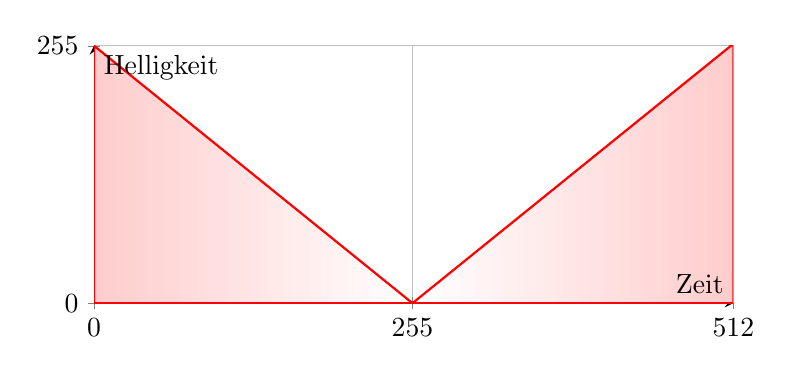
\begin{tikzpicture}
    \begin{axis}[
      axis lines=middle,
      xlabel={Zeit},
      ylabel={Helligkeit},
      xtick={0, 255, 512},
      xticklabels={0, 255, 512},
      ytick={0, 255},
      yticklabels={0, 255},
      extra x ticks = {0},
      extra y ticks = {0},
      ymin=0,
      ymax=255,
      xmin=0,
      xmax=512,
      width=.8\textwidth,
      height=.4\textwidth,
      grid=both,
    ]
      % \addplot[domain=0:512, samples=513, smooth, thick, blue] {\x < 256 ? 255-\x : \x-255};
      % red fill unter line according to value of x, 
      % \addplot[domain=0:512, samples=513, smooth, thick, red, fill=red!20] {255-\x} \closedcycle;
      % fill with linear gradient fading out to white at the end
      \addplot[domain=0:255, samples=513, smooth, thick, red, 
        shading = axis, left color=red!20, right color=white] {255-\x} \closedcycle;
      \addplot[domain=256:512, samples=513, smooth, thick, red,
        shading = axis, left color=white, right color=red!20] {\x-255} \closedcycle;
    \end{axis}
  \end{tikzpicture}
\end{center}

\begin{instruction}
  \begin{itemize}
    \item Baue die Schaltung auf.
    \item Probiere den Code aus.
    \item Setze alle Lampen auf Blau.
    \item Kannst du einen Farbverlauf von Blau zu Rot erzeugen?
    \item Was passiert, wenn du D2 nicht mit dem ersten Neopixel sondern in der Mitte mit einem DIN Pin verbindest? Nutze hierfür ein anderes Kabel.
    \item Kannst du trigonometrische Funktionen nutzen, um das Aufleuchten glätter zu machen?
  \end{itemize}
\end{instruction}

\begin{center}
  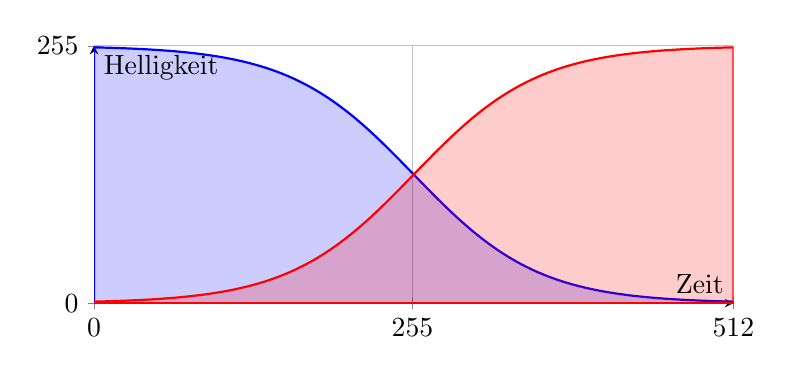
\begin{tikzpicture}
    \begin{axis}[
      axis lines=middle,
      xlabel={Zeit},
      ylabel={Helligkeit},
      xtick={0, 255, 512},
      xticklabels={0, 255, 512},
      ytick={0, 255},
      yticklabels={0, 255},
      extra x ticks = {0},
      extra y ticks = {0},
      ymin=0,
      ymax=255,
      xmin=0,
      xmax=512,
      width=.8\textwidth,
      height=.4\textwidth,
      grid=both,
    ]
    % sigmoid blue down from 255 to 0, fill transparent blue
    \addplot[domain=0:512, samples=513, smooth, thick, blue,
      fill=blue, fill opacity=0.2
    ] {255/(1+exp(0.02*(\x-256)))} \closedcycle;
    % sigmoid red up from 0 to 255
    \addplot[domain=0:512, samples=513, smooth, thick, red,
      fill=red, fill opacity=0.2
    ] {255/(1+exp(-0.02*(\x-256)))} \closedcycle;
    \end{axis}
  \end{tikzpicture}
\end{center}

|FastLED| definiert viele Funktionen, um Farben zu setzen\footnote{\url{https://fastled.io/docs/group___color_fills.html}}.
Beispielsweise füllt |fill_solid(led, NUM_LEDS, CRGB::Goldenrod);| alle LEDs mit der Farbe Goldgelb.
Andere Funktionen wie |fill_gradient_RGB(led, NUM_LEDS, CRGB::Red, CRGB::Blue);| können einen Farbverlauf zwischen bis zu vier Farben erzeugen.\footnote{Beispiel: \url{https://wokwi.com/projects/394601469488062465}}
Es gibt auch zugehörigen |fill_gradient| Funktionen, die im \hrefnote{https://en.wikipedia.org/wiki/HSL_and_HSV}{HSV} statt RGB Farbraum arbeiten.

Jetzt wollen wir unsere LEDs mit dem Potentiometer verbinden.
\begin{instruction}
  \begin{itemize}
    \item Entwirf eine Schaltung, die die Potentiometer Einstellung misst.
    \item Füge die LED Leiste in die Schaltung ein.
    \item Schalte entsprechend der Potentiometer Einstellung viele LEDs an. Bei $\SI{50}{\percent}$ sollten $5$ der $10$ LEDs leuchten.
    \item Färbe die aktiven LEDs in einem Farbverlauf von Rot über Gelb nach Grün ein.
  \end{itemize}
\end{instruction}


\section*{Potentiometer Verwenden}

Zum Auslesen funktioniert unser Potentiometer gut.
Allerdings ist der Widerstand für die meisten Anwendungen zu hoch.

Aber wir können den Widerstand verringern, indem wir einen Widerstand parallel schalten.
Erinnere dich daran, dass Parallelwiderstände sich nach dem Kehrwert der Summe der Kehrwerte addieren.
\[
  R_{\text{gesamt}} = \frac{1}{\left( \frac{1}{R_1} + \frac{1}{R_2} \right)}
\]

\sidebyside{poti2}

Eine kurze Rechnung ergibt, dass wir mit einem $S\SI{100}{\kohm}$ Potentiometer und einem $\SI{1}{\kohm}$ Widerstand
ein maximalen Wert von circa $\SI{990}{\ohm}$ erreichen.
Wir haben das Potentiometer also auf circa $\SI{1}{\kohm}$ verringert.
Jedoch haben wir dabei auch die Kurve des Potentiometers verändert.

Schauen wir uns dafür den Gesamtwiderstand beim Drehen des Potentiometers an:
\begin{center}
  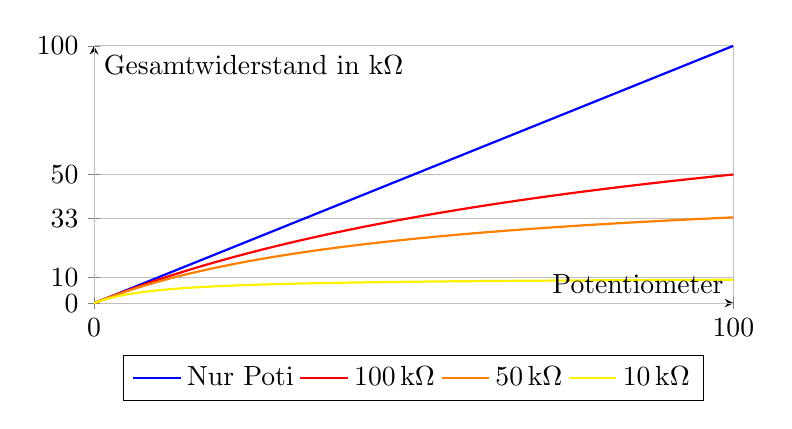
\begin{tikzpicture}
    \begin{axis}[
      axis lines=middle,
      xlabel={Potentiometer},
      ylabel={Gesamtwiderstand in $\si{\kohm}$},
      xtick={0, 100},
      xticklabels={0, 100},
      ytick={0, 10, 33, 50, 100},
      yticklabels={0, 10, 33, 50, 100},
      extra x ticks = {0},
      extra y ticks = {0},
      ymin=0,
      ymax=100,
      xmin=0,
      xmax=100,
      width=.8\textwidth,
      height=.4\textwidth,
      grid=both,
      legend style={at={(0.5,-0.2)},anchor=north},
      % labels next to each other instead of below
      legend columns=-1,
    ]
    % 100kOhm
    % 50kOhm
    % 10kOhm
    \addplot[domain=0:100, samples=100, smooth, thick, blue]
      {\x};
    \addlegendentry{Nur Poti}
    \addplot[domain=0:100, samples=100, smooth, thick, red]
      {1/(1/100 + 1/\x)};
    \addlegendentry{$\SI{100}{\kohm}$}
    \addplot[domain=0:100, samples=100, smooth, thick, orange]
      {1/(1/50 + 1/\x)};
    \addlegendentry{$\SI{50}{\kohm}$}
    \addplot[domain=0:100, samples=100, smooth, thick, yellow]
      {1/(1/10 + 1/\x)};
    \addlegendentry{$\SI{10}{\kohm}$}
    \end{axis}
  \end{tikzpicture}
\end{center}
Wir erreichen deutlich geringere Widerstände aber unsere Kurve nimmt eine logarithmische Form an.
Der Widerstand ist länger hoch und fällt dann steil ab.
Wenn wir den Widerstand halbieren wollen ist das kein Problem, aber wenn wir den Widerstand auf ein Zehntel verringern wollen, wird unser Potentiometer
praktisch konstant.

Bei einigen Anwendungen kann ein Nicht-lineares Verhalten gewünscht sein.
Beispielsweise bei Lautstärkereglern oder Dimmern.
Damit ein Geräusch doppelt so laut klingt, muss die Lautstärke nicht verdoppelt werden, sondern verzehnfacht werden.


\section*{Ausblick}

Jetzt hast du die wichtigsten Grundlagen und ein Haufen Zusatzinformationen, 
die hoffentlich interessant waren, gelernt.
Damit bist du bereit viele eigene Projekte dir auszudenken und umzusetzen.

Ein paar Zusatzmaterialien sind bereits vorhanden, sodass du mit den ersten 
Projekten direkt loslegen kannst.

Hier sind ein paar Anreize für eigene Projekte:
% checkbox list
\begin{itemize}[label=\textsquare]
  \item Schafe zählen permanent.
  Aktuell wird der Zähler unserer Schafe bei jedem Reset (Strom aus und wieder an oder Übertragen) zurückgesetzt.
  Der Arduino verfügt über einen internen $\SI{1}{\kilo\byte}$ EEPROM Speicher, der auch nach einem Reset erhalten bleibt.
  Damit kannst du die Schafe zählen und den Zähler speichern.
  Beim Start lädst du den Zähler und zählst weiter.
  \item Schafe animieren.
  Aktuell haben wir nur Schafe per serieller Kommunikation angezeigt.
  Kannst du die Schafe animieren?
  Einerseits eine kleine Text Animation bei der Kommunikation.
  Oder andererseits mit dem LED Streifen.
  \item Mit Knöpfen kann man viel machen.
  Du kannst dir deinen eigenen Controller bauen.
  Oder auch eine Minitastatur.
  Probiere aus einen Knopf anzuschließen. Stell sicher, dass keine Direktverbindung zwischen VCC und GND besteht,
  indem du einen Widerstand dazwischen schaltest.
  Je nachdem wie du die Schaltung aufbaust, wirst du im offenen Zustand 5V oder 0V sehen und umgekehrt im geschlossenen Zustand.
  Das hängt von der genauen Verkabelung und Position der Widerstände ab.
  Je nach Anwendungsfall ist das eine oder das andere besser.
  Lies hierzu auch über sogenannte \hrefnote{https://en.wikipedia.org/wiki/Pull-up_resistor}{Pullup und Pulldown Widerstände}.
  \item Wenn man viele Knöpfe hat, gehen schnell die Pins aus.
  Kannst du eine Matrix bauen, um viele Knöpfe mit wenigen Pins anzusteuern?
  Lies auch über Multiplexing und Charlieplexing. Das sind weitere, etwas kompliziertere, 
  Techniken, um viele Pins zu sparen.
  Es gibt noch einen weiteren Weg, mit dem du über einen (analogen) Pin viele Knöpfe lesen kannst.
  Kannst du herausfinden, wie das geht?
  \item LEDs können auch als Solarzellen genutzt werden.
  Jede LED ist auch eine Solarzelle. Bei Licht produziert sie Strom.
  Lies den Strom mit einem analogen Pin aus.
  Du wirst feststellen, dass einige Schwankungen vorhanden sind.
  Wenn du deine Ausgabe zu |Serial.print("A0: "); Serial.println(analogRead(A0));| änderst, kannst du die Werte im SerialPlotter sehen.
  Kannst du damit herausfinden, wann die LED Licht sieht und wann nicht?
  \item Es gibt noch weitere Kommunikationsmodi zwischen Hardware Bauteilen.
  Informiere dich über SPI, I2C und UART.
  \item Schau dir die Beispielprogramme unter Datei $\rightarrow$ Beispiele an.
  Da sind viele nützliche Programme und Erklärungen.
\end{itemize}

Viel Spaß beim Basteln!

\section*{Referenzen}

Im Folgenden sind ein paar interessante Links für die weitere Recherche zusammengestellt:

\begin{itemize}
  \item \hrefnoteinline{https://docs.arduino.cc/learn/}{Dokumentation zum Arduino}
  \item \hrefnoteinline{https://docs.arduino.cc/programming/}{Dokumentation zum Programmieren}
  \item \hrefnoteinline{https://wokwi.com/projects/new/arduino-nano}{Web IDE mit Simulation}
  \item \hrefnoteinline{https://create.arduino.cc/editor}{Web IDE (braucht Account)}
  \item \hrefnoteinline{https://raydiy.de/arduino-esp32-programmieren-mit-platformio-und-visual-studio-code/}{Blog über VSCode Plugin (PlatformIO)}
  % \item \hrefnoteinline{}{}
\end{itemize}

Weitere Referenzen:
\begin{itemize}
  \item \hrefnoteinline{https://de.wikipedia.org/wiki/Liste_der_Schaltzeichen_(Elektrik/Elektronik)}{Liste der Schaltzeichen elektronischer Bauteile}
  \item \hrefnoteinline{https://raydiy.de/neopixel-mit-arduino-und-esp32-der-led-streifen-ultra-guide/}{Neopixel LED Streifen Guide}
  \item \hrefnoteinline{https://playground.arduino.cc/uploads/Main/arduino_comic_v0004/index.pdf}{Webcomic}
  \item \hrefnoteinline{https://fritzing.org/}{Designprogramm von Schaltungen mit vielen Bauteilen. Kann auch Diagramme und PCBs erstellen.}
  \item \hrefnoteinline{http://www.cburch.com/logisim/}{Simulationstool für logische Schaltkreise mit Gattern}
  \item \hrefnoteinline{https://www.kicad.org/}{Programm für Schaltpläne und PCBs}
  \item \hrefnoteinline{https://www.tinkercad.com/dashboard}{Website für Simulation und Schaltpläne. Skratch-ähnliche Programmierumgebung, aber kein Arduino Nano (dafür Arduino Uno).}\footnote{Blog: \url{https://www.tinkercad.com/blog/official-guide-to-tinkercad-circuits}}
\end{itemize}

\section*{Wörterbuch}
Im Internet findet man meist mehr und bessere Informationen auf Englisch.
Insbesondere ist die universelle Sprache für Programme Englisch.
Hier sind Übersetzungen einige wichtige Wörter:
\begin{itemize}
  \item \hrefnoteinline{https://de.wikipedia.org/wiki/Steckplatine}{Steckbrett/Steckplatine: Breadboard}
  \item \hrefnoteinline{https://de.wikipedia.org/wiki/Elektrischer_Widerstand}{Widerstand: Resistor}
  \item \hrefnoteinline{https://de.wikipedia.org/wiki/Kondensator_(Elektrotechnik)}{Kondensator: Capacitor}
  \item \hrefnoteinline{https://de.wikipedia.org/wiki/Potentiometer}{Potentiometer: Potentiometer}
  \item \hrefnoteinline{https://de.wikipedia.org/wiki/Transistor}{Transistor: Transistor}
  \item \hrefnoteinline{http://www.geofex.com/article_folders/potsecrets/potscret.htm}{Blog about Potentiometer und Widerstandkurven} % http://www.geofex.com/
\end{itemize}

\section*{Zusatzmaterial}
Auf Kondensatoren steht die Kapazität in Farad $\si{\farad}$.
Aber auf Widerständen steht nichts.
Stattdessen haben sie eine Farbcodierung.
Die ersten Ringe geben einen Faktor an, der vierte (oder generell vorletzte) die Größenordnung und der letzte die Toleranz:

\begin{center}
\includegraphics[width=.8\textwidth]{images/bauteil_widerstand_kennzeichnung.png}
\end{center}


\end{document}
